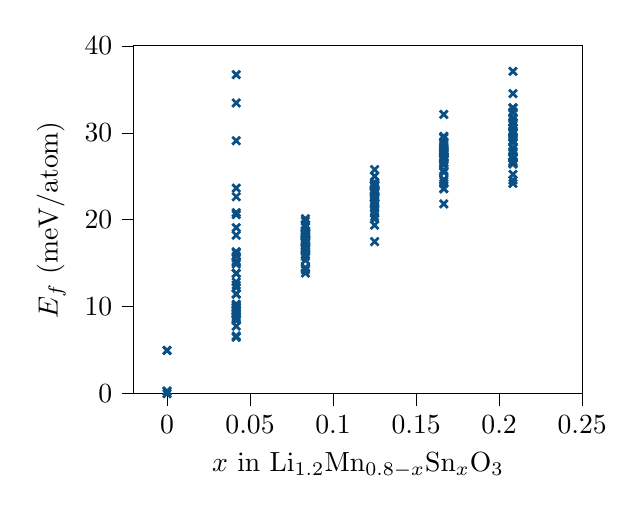
\begin{tikzpicture}

\begin{axis}[
width=0.6\textwidth, height=6cm,
tick align=outside,
tick pos=left,
xmin=-0.02, xmax=0.25,
xtick={0, 0.05, 0.1, 0.15, 0.2, 0.25},
xticklabels={0, 0.05, 0.1, 0.15, 0.2, 0.25},
x grid style={white!69.0196078431373!black},
xlabel={$x$ in Li$_{1.2}$Mn$_{0.8-x}$Sn$_x$O$_3$},
xtick style={color=black},
ymin=0, ymax=40,
ytick={0, 10, 20, 30, 40},
yticklabels={0, 10, 20, 30, 40},
y grid style={white!69.0196078431373!black},
ylabel={$E_f$ (meV/atom)},
ytick style={color=black}, mark options={line width=1pt},
legend style={
at={(1, 1)}, anchor=north east, draw=none, fill=none, 
},
]
% This file was created by tikzplotlib v0.9.1.
\definecolor{color0}{rgb}{0.0392156862745098,0.313725490196078,0.52156862745098}

\addplot [only marks, mark=x, draw=color0, fill=color0, colormap/viridis]
table{%
x                      y
0 0
0 0.31117166666661
0 4.98020927083331
0 4.97478093749848
0 0.265032395832421
0.0416666666666667 15.2386898248987
0.0416666666666667 16.3269272207326
0.0416666666666667 20.5887670123978
0.0416666666666667 19.0977287832307
0.0416666666666667 20.8145852415643
0.0416666666666667 13.8410470123979
0.0416666666666667 8.8071136790645
0.0416666666666667 12.2127350332316
0.0416666666666667 8.43711711656525
0.0416666666666667 36.6861954498986
0.0416666666666667 6.6397675332307
0.0416666666666667 14.9104065957327
0.0416666666666667 11.4367493040649
0.0416666666666667 18.2227631582325
0.0416666666666667 2473.30455555406
0.0416666666666667 334.185957116565
0.0416666666666667 9.06490472073174
0.0416666666666667 15.1117193040654
0.0416666666666667 9.96965951239759
0.0416666666666667 8.60172638739798
0.0416666666666667 2520.53488586657
0.0416666666666667 15.8029944082322
0.0416666666666667 13.8394555540638
0.0416666666666667 12.8477562832315
0.0416666666666667 29.087034512398
0.0416666666666667 9.1810585748987
0.0416666666666667 10.1848557623977
0.0416666666666667 7.76613992906505
0.0416666666666667 8.60846419989791
0.0416666666666667 6.48778159573127
0.0416666666666667 10.2949804498983
0.0416666666666667 9.6029285748972
0.0416666666666667 22.6482043040647
0.0416666666666667 16.191564304065
0.0416666666666667 33.4274344082327
0.0416666666666667 12.4913215957313
0.0416666666666667 11.4895589915643
0.0416666666666667 1294.46220784573
0.0416666666666667 9.53851347073098
0.0416666666666667 1225.43296315823
0.0416666666666667 9.54966815823177
0.0416666666666667 23.638893366564
0.0416666666666667 3565.83250534573
0.0416666666666667 9.84547690823156
0.0416666666666667 9.94626607489934
0.0833333333333333 16.656766003962
0.0833333333333333 18.4626720456296
0.0833333333333333 16.8090592331291
0.0833333333333333 18.6703513164626
0.0833333333333333 18.1682511081294
0.0833333333333333 18.0458325664612
0.0833333333333333 17.3863199622952
0.0833333333333333 20.117021941463
0.0833333333333333 17.684096628962
0.0833333333333333 18.1234626706284
0.0833333333333333 18.7221944414626
0.0833333333333333 17.375109962295
0.0833333333333333 19.1593700664614
0.0833333333333333 15.3439350664615
0.0833333333333333 19.4292735039616
0.0833333333333333 14.488057774795
0.0833333333333333 16.9598531914625
0.0833333333333333 14.2287780872954
0.0833333333333333 15.7892975664622
0.0833333333333333 17.8882036081289
0.0833333333333333 17.953737878962
0.0833333333333333 17.6843527747954
0.0833333333333333 17.6074251706277
0.0833333333333333 18.4113550664622
0.0833333333333333 14.4141539206279
0.0833333333333333 13.8719118372956
0.0833333333333333 16.3145022539626
0.0833333333333333 15.9794942331291
0.0833333333333333 16.5889231914618
0.0833333333333333 16.4368435039608
0.0833333333333333 16.7142223581289
0.0833333333333333 19.3360607956274
0.0833333333333333 18.5732875664615
0.0833333333333333 19.8479183997942
0.0833333333333333 18.432045170629
0.0833333333333333 18.2946247539617
0.0833333333333333 16.3892895456288
0.0833333333333333 17.4936399622949
0.0833333333333333 18.2565055872959
0.0833333333333333 18.3334969414626
0.125 24.3105868705267
0.125 23.5059885371913
0.125 23.9258930163593
0.125 23.3498340580254
0.125 24.1912675996931
0.125 23.8893111413598
0.125 23.4280898913588
0.125 22.6777135371914
0.125 22.499776037193
0.125 22.1307042663592
0.125 21.8831239538591
0.125 23.9304347871925
0.125 23.1168334330252
0.125 23.947960724692
0.125 23.106370828859
0.125 23.409997078859
0.125 24.1138111413579
0.125 24.0050514538583
0.125 20.3486212455259
0.125 17.4866664538587
0.125 23.3119515580245
0.125 22.5319798913595
0.125 22.5026360371916
0.125 22.2292011413585
0.125 20.0877454121922
0.125 22.5481289538592
0.125 24.1253675996922
0.125 21.7470766621921
0.125 23.9000336413588
0.125 23.1665066621924
0.125 23.049980828858
0.125 23.9220918705256
0.125 23.2004475996912
0.125 20.7222964538594
0.125 20.8799168705265
0.125 21.3070517663598
0.125 21.8364700996925
0.125 25.0085330163592
0.125 25.7633991621922
0.125 19.379074370526
0.166666666666667 29.5897805495922
0.166666666666667 28.9658649245914
0.166666666666667 29.4282298204247
0.166666666666667 28.589117528758
0.166666666666667 28.8527641954253
0.166666666666667 27.1768472162583
0.166666666666667 28.1529396120912
0.166666666666667 27.9507608620917
0.166666666666667 27.0616686745924
0.166666666666667 28.051189507925
0.166666666666667 26.5412230495925
0.166666666666667 26.5753132579252
0.166666666666667 28.3969500287582
0.166666666666667 26.995791799592
0.166666666666667 24.4523859662578
0.166666666666667 21.8240141954253
0.166666666666667 23.5887031537572
0.166666666666667 24.159376278758
0.166666666666667 27.8743114870905
0.166666666666667 27.6722000287584
0.166666666666667 27.2112473204245
0.166666666666667 26.5492359662587
0.166666666666667 27.5873806537574
0.166666666666667 27.2332212787574
0.166666666666667 26.952836695425
0.166666666666667 25.4591486745919
0.166666666666667 27.5099319037593
0.166666666666667 27.5955348204255
0.166666666666667 26.7783336745917
0.166666666666667 23.5582121120905
0.166666666666667 27.9472236745923
0.166666666666667 25.5427305495917
0.166666666666667 25.7032762787595
0.166666666666667 27.7170583620907
0.166666666666667 24.6330739870912
0.166666666666667 27.2060858620917
0.166666666666667 27.9349440912582
0.166666666666667 32.1147976329246
0.166666666666667 26.296553362092
0.166666666666667 27.0430035704243
0.208333333333333 34.5013809994899
0.208333333333333 32.3486400619895
0.208333333333333 24.550888707823
0.208333333333333 27.8125543328236
0.208333333333333 28.2904161036561
0.208333333333333 28.8855487078226
0.208333333333333 27.0703182911567
0.208333333333333 26.4052621453224
0.208333333333333 26.5056138119895
0.208333333333333 24.1766436036559
0.208333333333333 27.8631812078216
0.208333333333333 27.0300987078236
0.208333333333333 32.8819201661559
0.208333333333333 31.5738886036558
0.208333333333333 31.1915719369895
0.208333333333333 30.010899853655
0.208333333333333 30.1398297494884
0.208333333333333 30.2911651661559
0.208333333333333 30.0623625619898
0.208333333333333 29.4394358953229
0.208333333333333 27.3426104786565
0.208333333333333 29.0714241244898
0.208333333333333 29.0610415203232
0.208333333333333 30.61190537449
0.208333333333333 27.8186945411565
0.208333333333333 31.2032990203224
0.208333333333333 31.198784541155
0.208333333333333 37.0649009994888
0.208333333333333 27.8186638119897
0.208333333333333 29.4655033953233
0.208333333333333 26.4986570411572
0.208333333333333 26.706616728656
0.208333333333333 31.7379253744892
0.208333333333333 29.9113002703222
0.208333333333333 27.2624965203234
0.208333333333333 32.8356161036552
0.208333333333333 32.3944814161563
0.208333333333333 31.2283648536549
0.208333333333333 25.2170041244901
0.791666666666667 123.123494798062
0.791666666666667 119.865812506394
0.791666666666667 120.188594902228
0.791666666666667 143.354342714726
0.791666666666667 114.716814068894
};

\end{axis}

\end{tikzpicture}
